\documentclass{article}
\usepackage{ifxetex}
\ifxetex
  \usepackage{fontspec}
\else
  \usepackage[T1]{fontenc}
  \usepackage[utf8]{inputenc}
  \usepackage{lmodern}
  \usepackage{float}
  \usepackage{graphicx} 
  \usepackage{morefloats}
  \usepackage{wrapfig}
  \usepackage{babel}
  \usepackage{enumerate}
\fi
  
\begin{document}
\begin{titlepage}
\begin{center}
    \vspace*{-1in}
    \begin{figure}[htb]
    \begin{center}
    
\includegraphics[width=8cm]{escudo-gde-trans.png}
    \end{center}
\end{figure}    
\begin{center}
LICENCIATURA EN FÍSICA \\
\vspace*{0.15in}
DEPARTAMENTO DE FÍSICA \\
\vspace*{0.6in}
\begin{large}
FÍSICA COMPUTACIONAL 1 \\
\end{large}
\vspace*{0.2in}
\rule{80mm}{0.1mm}\\
\vspace*{0.1in}
\begin{large}
\textbf{Reporte 5\\ }
\end{large}
\vspace*{0.3in}
\begin{large}
Alumna: \\
\vspace*{0.1in}
Brambilla Zamorano Fátima Fernanda\\
\end{large}
\vspace*{0.3in}
\rule{80mm}{0.1mm}\\
\vspace*{0.1in}
\begin{large}
Fecha: \\ 05/03/18\\
\end{large}
\end{center}
\end{center}
\end{titlepage}

\section{Introducción}
Continuando las actividades de la sesión 4, para esta nueva actividad continuamos trabajando con emacs, y los nuevos comandos que habiamos aprendido, así mismo, retomamos las actividades en Python por medio del uso de Jupyter. 
Esta actividad la empezamos partiendo de los últimos puntos en la actividad 4, donde se nos pedía hacer un script que juntara los datos mensuales del año 2017, y que nos dejara únicamente las lineas con las variables deseadas, entre ellas la estación de donde se obstuvieron los datos, la variable CAPE, la cual explicaremos más adelante, el agua precipitada, entre otras. 


\section{Fundamentos}
Parte fundamental de esta actividad recae en conocer los datos que trabajaremos, como lo son las variables CAPE y PW, las cuales explicaremos a continuación: 
\begin{itemize}
\item CAPE \\ La variable cape, \textit{Energía Potencial Convectiva Disponible} corresponde a una sección que llamaremos \textit{Air Motion}, y esta es una medida de inestabilidad a través de la \textit{profundidad de la atmósfera} y esta relacionada con la fuerza de corrientes ascendentes en tormentas eléctricas. ESta define la cantidad de energía (en una porción de aire) que esta disponible para la convección, y es proporcional a la máxima velocidad vertical potencial dentro de una corriente ascendente. Esta variable se mide en Joules/Kilogramo [J/Kg]. \\ Cuanto mayor sea el valor, mayor será el potencial el clima severo como tormentas eléctricas.
\item PW \\ O en español, AP, esta variable índica el agua precipitable. La precipitación es el deposito de agua de la superficie de la Tierra, en forma de lluvia, granizo, nieve o hielo. Todos los valores de precipitación se expresan en milimetros [mm] de liquido equivalente de agua para el intervalo de tiempo anterior (o pulgadas). Un milimetro de lluvia corresponde a un litro de agua por metro cuadrado de superficie o alrededor de 10mm de nieve.  
\end{itemize}
\section{Prodecimiento}
Del archivo que habíamos creado previamente, aquel que contenia varias variables distintas, así como la estación de la cual fueron recogidos los datos, extraimos por medio de los comandos cat y egrep los datos de la fecha, estación, CAPE y agua precipitada, creando un nuevo archivo. De ahí creamos una carpeta nueva, llamada \textit{Actividad5} para trabajar en ella, moviendo el archivo recien creado a esta. 
Lo siguiente fue extraer de este último archivo, los datos para las horas marcadas con 00Z, y 12Z en dos archivos distintos, para cual se utilizo un script nuevo: 

\begin{figure}[htb]
    \begin{center}
    \includegraphics[width=8cm]{script00zcontenido.png}
    \end{center}
\end{figure}

En la imagen anterior, se muestra el comando utilizado para obtener los dos nuevos archivos a partir de uno solo, y en un único script. Y una vez que tuvimos ambos archivos en la carpeta de trabajo, pasamos a editar cada uno de ellos, para quitar la información innecesaria de las lineas, dejando únicamente los valores de las fechas, cambiando los meses por su equivalente númerico, y los datos númericos de las variables CAPE y agua precipitada. 
Posteriormente, leímos ambos archivos de datos en \textit{Jupyter Notebook}

\section{Analsis de Datos}
Para analizar los datos, primero abrimos \textit{Jupyter Notebook} por medio de la terminal, y una vez editado el campo de trabajo en \textit{Python}, importamos las bibliotecas de pandas numpy y datetime para poder trabajar con ambos archivos de datos. Lo siguiente fue leer los archivos de datos, en una o dos celular de codigo, e indicarle al programa que ignorara los errores entre las lineas, es decir, que no tomará en cuenta las lineas en las que faltaran datos, o ignorara la ausencia de estos, también nos aseguramos que los datos fueran leidos correctamente antes de empezar a hacer gráficas para apreciar la distribución de los datos mensuales. \\
Se hicieron cuatro gráficas para cada archivo de datos, por lo que se obtuvieron cuatro pares de gráficas en total, las cuales compararemos más adelante. \\
Cabe mencionar que en el caso de dos de ellas, no puedo asegurar tener una buena explicación para el comportamiento que tienen, pues en realidad ni siquiera estoy segura de cual es el significado en las dos gráficas finales. \\

\section{Resultados} 

Las gráficas obtenidas para  los datos de los archivos de datos de las horas \textit{00Z y 12Z} se muestran a continuación. En primer lugar presentare las gráficas para la variable CAPE, las cuales quedaron de la siguiente manera:  \\
\\
\\ 
\\ 
\begin{figure}[htb]
    \begin{center}
    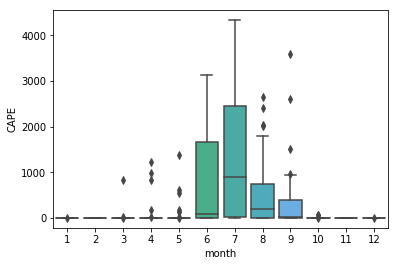
\includegraphics[width=8cm]{BoxPlot00z.png} 
    \end{center}
\end{figure}

\begin{figure}[htb]
    \begin{center}
    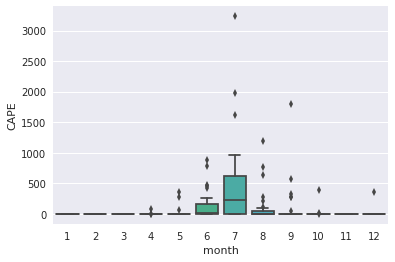
\includegraphics[width=8cm]{BoxPlot12Z.png} 
    \end{center}
\end{figure}

Los dos son gráficos de caja, el primero corresponde al archivo de las horas 00Z, y el segundo a las horas 12Z. Estas gráficas son de la variable CAPE en función del mes. En cambos casos podemos ver que los datos de los meses Junio, Julio y Agosto, y en caso de la primera gráfica, Septiembre también, son más extensos, de forma que se pueden apreciar las "cajas", sin embargo, los datos para las horas 00Z son más extensos que en el caso de las horas 12Z, por lo que los diagramas del primer gráfico son más grandes, y la dispersion en sus datos también, lo que ocasiona que los cuartiles de cada mes de datos sean de dinstinto tamaño. En el caso de las horas 12Z, la distribución de sus datos es menos extensa, de modo que las cajas que se aprecian en esta gráfica son más compactas. \\

El siguiente par de gráficas corresponden a los datos del agua precipitada en función del mes, estos también están en diagramas de caja, sin embargo, estos datos muestran una distribución más sencilla de apreciar que las gráficas para la variable CAPE. De nueva cuanta, la primera gráfica corresponde a las horas 00Z, mientras que la segunda es de las horas 12Z. \\
\\ 

\begin{figure}[htb]
    \begin{center}
    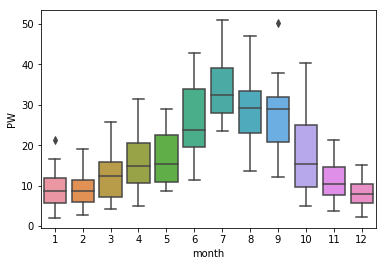
\includegraphics[width=8cm]{BoxPlotSea00Z.png} 
    \end{center}
\end{figure}

\begin{figure}[htb]
    \begin{center}
    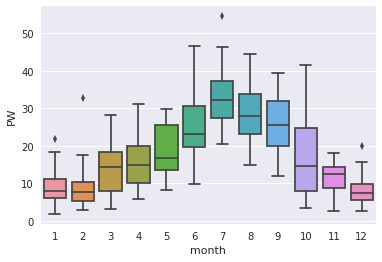
\includegraphics[width=8cm]{BoxPlotS12Z.png} 
    \end{center}
\end{figure}

La diferencia entre estas dos, no es tan apreciable como en el caso anterior, aunque esto no quiere decir que sean iguales, pues en realidad se puede apreciar la diferencia en los meses de Mayor, Junio, y Julio, donde los diagramas de caja muestran una diferencia mayor que en los otros meses. Para las horas 00Z los datos son más dispersos que para las horas 12Z en el caso de la variable PW. \\ 

En las gráficas que se mostraran más adelante se puede ver una dispersión mayor en los datos de la primera, y una más comprida para la segunda, aunque en ambos casos es una recta la curva que mejor se ajusta a los datos.   \\ 
\\ 
\begin{figure}[htb]
    \begin{center}
    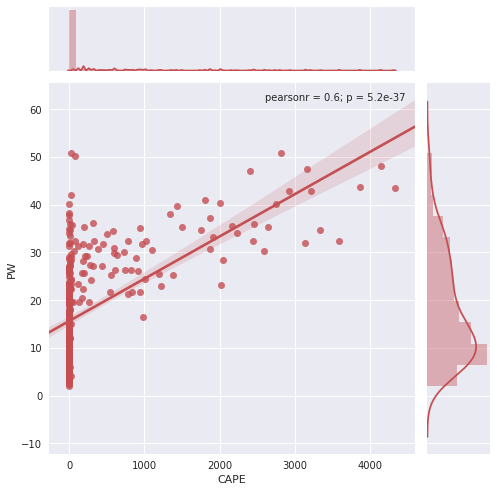
\includegraphics[width=8cm]{Seaborn00z.png} 
    \end{center}
\end{figure}

\begin{figure}[htb]
    \begin{center}
    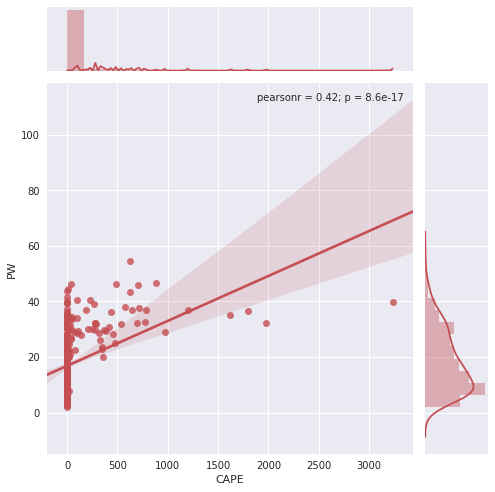
\includegraphics[width=8cm]{Seaborn12Z.png} 
    \end{center}
\end{figure}

Por último, se presetan dos gráficas que muestran un comportamiento especial para los meses de marzo, y octubre, el primer caso corresponde a la gráfica de las horas 00Z y el según a las horas 12Z \\ 

\begin{figure}[htb]
    \begin{center}
    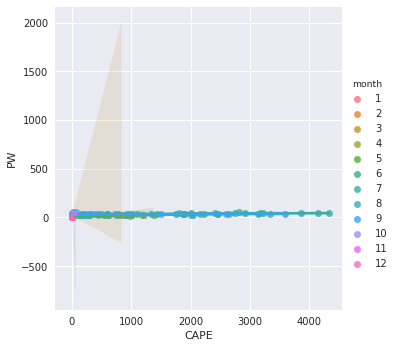
\includegraphics[width=8cm]{GFinal00z.png} 
    \end{center}
\end{figure}

\begin{figure}[htb]
    \begin{center}
    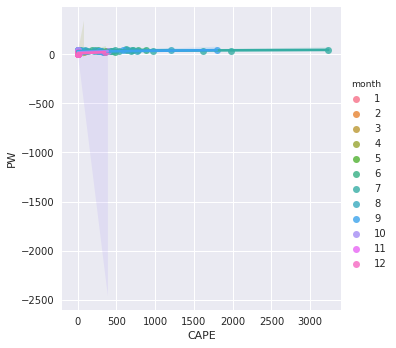
\includegraphics[width=8cm]{GFinal12Z.png} 
    \end{center}
\end{figure}

Es importante mencionar que para el caso del primer gráfico, el mes de Marzo se exntiende hacia el lado positivo en la variable PW, mientras que para el mes de octubre, PW se extiende hacia el lado negativo. 


\section{Conclusiones}
Para realizar esta actividad era necesario saber manejar emacs, y conocer varios de los comandos que se utilizan en su entorno de trabajo, ya que no solo nos debiamos apoyar en distintos scripts para poder realizar las actividades pedidas, sino que debíamos depurar los archivos obtenidos para eliminar la información innecesaria de estos últimos, de modo que habría sido imposible completar la actividad sin saber nada del editor emacs. Así mismo, debiamos estar familiarizados con la manera de trabajar en Jupyter Notebook, ya que la lectura de datos era una parte importante de la práctica, de tal manera que, sino conocieramos la forma en que se trabaja en Python no habríamos sido capaces de acabar con la actividad de la semana. 
Esto quiere decir que, en definitiva es necesario seguir un orden lógico y práctico en las actividades, y no saltar de una a otra y luego devolverse a una anterior, pues las nuevas actividades siempre dependeran de los conocimientos adquiridos en las pasadas.  

\section{Bibliografía}
\begin{enumerate}
\item meteoblue . (s.f.). Obtenido de https://content.meteoblue.com/es/ayuda/variables-meteorologicas
\end{enumerate}

\section{Ápendice}
\begin{itemize}
\item ¿Cómo se te hizo esta actividad? ¿Compleja, Difícil, Sencilla? \\ Esta actividad me parecio similar a la anterior, es decir, tuve alguna que otra dificultad para al empezar, sobre todo para pensar en como hacer los scripts en los que me apoye, aunque al final terminaron siendo bastantes sencillos de hacer. Para mi la actividad en realidad es sencilla, solo requiere que se tengan conocimientos previos de como trabajar en emacs.  
\item ¿Qué te llamo másla atención? \\ Me gusto la idea de hacer scripts que nos ayudaran a crear nuevos archivos de datos, y la edición de estos últimos en emacs. 
\item¿Qué parte fue la que menos te interesó hacer? \\ No hubo una parte que no me pareciera interesante. 
\item Cómo mejorarías esta actividad? ¿Qué le faltó? ¿Qué sobró? \\ Considero que hace falta una explicación de las gráficas creadas en Python, saber que significa para poder explicarlas en el reporte de actividad. 
\item ¿Hasta este punto, que te parece el uso de Jupyter para programar en Python? \\ Hasta ahora me sigue pareciendo un entorno agradable para la programación. 
\end{itemize}

\end{document}
